\section{Case Studies}\label{sec:usecases}

In this section, we provide \numCases case studies demonstrating the practical
utility of heterogeneous FDE not achievable with prior work. We cover a wide
range of situations, highlighting concerns like meeting latency goals, trading
off security and writable space, and keeping within an energy budget, all
demonstrating the utility of both temporal and spatial switching strategies. All
experiments are repeated multiple times.


% ===========================================================
\subsection{Battery Saver Mode}\label{subsec:usecase-battery}

% About: motivation
In this first case study, we revisit the motivational example. Here, the mobile
device is ``forced'' to locally encrypt files with Freestyle Balanced Cipher
(``\cone'') for safely backing up the file to the backend cloud, but when the
battery saver mode is on, the device will switch to a more energy-efficient
cipher, ChaCha8 (``\ctwo''), and at the same time pausing the backup upload to
the cloud momentarily (\eg the company does not want files to be saved in the
cloud without \cone encryption. Our goal is to complete I/Os as much as we can
before the device dies.

% About: setup
To simulate I/O activity, we begin randomly writing 10 40MB files using the
Freestyle Balanced cipher for 2 minutes. After the first 5 seconds, the device
enters ``battery saver'' mode, which we simulate by underclocking the cores to
their lowest frequencies and using \texttt{taskset} to transition \sys processes
to the energy-efficient LITTLE cores. In this low battery mode, \sys switches to
the ChaCha8 cipher.

\hsg{I don't understand \cref{fig:usecase-battery}. You said after 5 seconds. we
switch to ChaCha8. But why the FB+ChaCha line is still going up? Why it doesn't
flat out like the ChaCha line?? and why do even need to show the ChaCha8 only
line?}

\def \hmina {\hspace{-0.1in}}
\def \hminb {\hspace{-0.2in}}

\def \fgw {2in}
\def \fgh {1in}

% \begin{floatingfigure}[r]{2in}  (and \end{..})

\begin{figure}[t]
    \centerline{
        % \hmina
        % \includegraphics[width=\fgw]{data/usecase-battery}
        % \hminb
        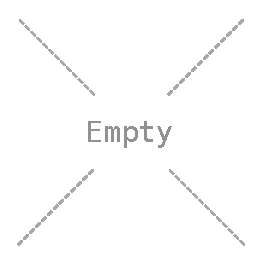
\includegraphics[height=\fgh]{empty.eps}
    }

    \mycaption{fig:usecase-battery}{Battery saver case}{Energy-security
    tradeoff given strict energy budget as discussed in
    \cref{subsec:usecase-battery}.}
\end{figure}

 \hsg{we should exlude ChaCha8 only, unless
you have a major point here}

% About: result
\cref{fig:usecase-battery} shows the time versus energy used. At 0 seconds, we
begin writing. At 5 seconds, the ``battery saver'' event occurs, causing the
system to be underclocked. At 120 seconds, the system will die. If we blow past
our energy ceiling, the system will die. The figure shows two lines:
%
{\bf (1)} {\em Freestyle Balanced only}, that favors security even when backups
are paused; the device dies before the I/Os complete.
%
{\bf (2)} {\em Freestyle Balanced $+$ ChaCha8}, that performs the switch when
the system enters the low power state. Our results show that, while the system
uses slightly more power in the short term, we stay within our energy budget and
finish before the devices dies.
%
When we get the device to a charger (not shown), the cloud backup is enabled
again and when the nuggets are read, \sys automatically converges them back to
Freestyle Balanced.

% About: overall result
On average, using forward switching resulted in a 3.3x total energy reduction
compared to exclusively using Freestyle Balanced, allowing us to remain within
our energy budget. \hsg{I don't see this 3.3x in the graph. Did you accidentally
label the lines incorrectly?}. We note, however, that the energy savings is not
the point of this experiment. Rather, the lesson learned is that \sys enables
the system to move to the right point in the energy/security tradeoff space so
that the current task can still be accomplished before the battery is drained
and without compromising backup security at any point.


% ================================================================
\subsection{Select Data Encryption}\label{subsec:usecase-agnostic}

% About: background
This use case illustrates utility of selective switching to achieve a
performance win---if only a small percentage of the data needs the strongest
encryption, then only a small percentage of the data should have that associated
overhead, while the rest can use a minimalist encryption. As mentioned before,
this feature requires users to annotate certain files with a special tag via
file system calls, which would then be stored in the inode. Because the \sys
layer is file oblivious, every block I/O through the \sys layer will be labeled
with the corresponding cipher.

% About: setup
We begin by with 10 5MB and 4KB write-read operations to two \sys drive
instances: one using ChaCha8 and the other using Freestyle Strong. They
represent two extreme where ChaCha8 is a low-latency cipher and Freestyle Strong
exhibits a very high overhead. We then run another \sys instance with a 7:3
ratio where 30\% of the data considered highly sensitive uses Freestyle Strong.

\def \hmina {\hspace{-0.1in}}
\def \hminb {\hspace{-0.2in}}

\def \fgw {2in}
\def \fgh {1in}

% \begin{floatingfigure}[r]{2in}  (and \end{..})

\begin{figure}[t]
    \centerline{
        % \hmina
        % \includegraphics[width=\fgw]{data/usecase-agnostic}
        % \hminb
        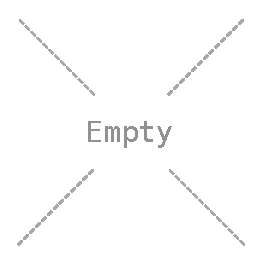
\includegraphics[height=\fgh]{empty.eps}
    }

    \mycaption{fig:usecase-agnostic}{Scalable encryption}{Filesystem-agnostic
    file-level encryption as discussed in \cref{subsec:usecase-agnostic}.}
\end{figure}


% About: outcome
The left-side and right-side bars in \cref{fig:usecase-agnostic} show the two
extremes; ChaCha8 exhibits a low latency, consistently less than 1 second across
the workloads, while Freestyle Strong exhibits 5 to 20 second latency depending
on the workload. The selective switching (middle bars) shows a reduction of 3.1x
to 4.8x for read latency and 1.6x to 2.8x for write latency, all without
compromising the security needs of the most sensitive data. Thus, selective
switching keeps our sensitive data at the mandated security level while keeping
the performance (and also battery life) benefits of using a fast cipher for the
majority of I/O operations.


% ===============================
\subsection{No-Downtime Encryption Upgrade}\label{subsec:usecase-upgrade}

\def \hmina {\hspace{-0.1in}}
\def \hminb {\hspace{-0.2in}}

\def \fgw {2in}
\def \fgh {1in}

% \begin{floatingfigure}[r]{2in}  (and \end{..})

\begin{figure}[t]
    \centerline{
        % \hmina
        % \includegraphics[width=\fgw]{usecase-upgrade}
        % \hminb
        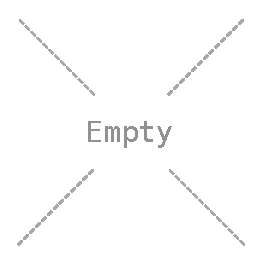
\includegraphics[height=\fgh]{empty.eps}
    }

    \mycaption{fig:usecase-upgrade}{Cipher upgrade without downtime}{Switching
    storage system encryption with zero downtime as discussed in
    \cref{subsec:usecase-upgrade}.}
\end{figure}


In \cref{fig:usecase-upgrade} \TODO{finish sentence}. \hsg{we must have a short
case study here. Otherwise no point of talking about mirrored switch}.
